\documentclass[a4paper,12pt]{book}
\usepackage{graphicx}
\usepackage[export]{adjustbox}
\usepackage{subcaption}
\graphicspath{{Pics/}}
\usepackage{charter}
\usepackage{fancyhdr}
\usepackage{enumerate}
\usepackage{enumitem}
\usepackage{siunitx}
\usepackage{amssymb}
\usepackage{longtable}
\usepackage{multicol}
\usepackage{multirow}
\usepackage{hhline}
\usepackage{parskip}
\setlength{\parskip}{6pt}
\usepackage{ragged2e}
\usepackage{geometry} %margin
\geometry{left=2.1cm,right=2.1cm,top=3cm,bottom=3cm}
\usepackage{setspace}
\SetSinglespace{1.2}
\singlespacing
\renewcommand{\ttfamily}{\fontfamily{pcr}\selectfont}
%\renewcommand{\familydefault}{\rmdefault}

\usepackage[,table]{xcolor}
\definecolor{LightBlue}{cmyk}{0.16,0.03,0.04,0}
\definecolor{Title}{cmyk}{0.8,0.1,0,0.3}
\setlength{\arrayrulewidth}{0.3mm}
\setlength{\tabcolsep}{2pt}
\setlength{\headheight}{15pt}
\renewcommand{\arraystretch}{1}
\usepackage{tikz}
\usepackage{nicematrix}
\newcommand*\circled[1]{\tikz[baseline=(char.base)]{\node[shape=circle,draw,inner sep=1pt] (char) {#1};}}

\newcolumntype{s}{>{\columncolor{Title}\RaggedLeft} m{3.5em}} % columntype for chapter title
\newcolumntype{d}{>{\columncolor{LightBlue}\RaggedRight} m{\textwidth}} % columntype for code bloc
\newcolumntype{a}{>{\columncolor{LightBlue}\RaggedRight} m{0.96\textwidth}} % columntype for secondary code bloc

\usepackage{titlesec}
\usepackage[hidelinks]{hyperref}
\urlstyle{same}

\captionsetup[figure]{labelsep=period,font={bf}}
\captionsetup[table]{font={bf},labelsep=period}

\newcommand{\titlename}{}

\newcommand{\chaptertitle}[2]{ %reset chapter format
\vspace{-120pt}
\gdef\titlename{#1}
{
\SetSinglespace{1.1}
\singlespacing
\Huge\bfseries
\setlength{\tabcolsep}{8pt}
\renewcommand{\arraystretch}{1.5}
\begin{tabular}{s >{\RaggedRight}m{14.5em}}
\textcolor{white}{Chapter\newline\thechapter}&\textcolor{Title}{#2}
\end{tabular}
}
}

\newcommand{\partpic}[1]{%insert picture
    \tikz[remember picture,overlay] \node at (current page.center){\includegraphics[width=\paperwidth]{#1}};
}

\titleformat{\part} %reset part %format
{\huge\bfseries} % format
{} % label
{0em} % sep
{\Centering} % before-code

\titleformat{\chapter} %reset chapter %format
{\huge\bfseries} % format
{} % label
{0em} % sep
{\Centering} % before-code
\titlespacing{\chapter}{0pt}{0pt}{0pt}

\titleformat{\section} %reset section %format
{\Large\bfseries} % format
{\textcolor{Title}{\thesection}} % label
{0.5em} % sep
{\color{Title}} % before-code
\titlespacing{\section}{0pt}{12pt}{6pt}

\titleformat{\subsection} %reset subsection %format
{\large\bfseries} % format
{\textcolor{Title}{\thesubsection}} % label
{0.5em} % sep
{\color{Title}} % before-code
\titlespacing{\subsection}{0pt}{8pt}{6pt}

\newenvironment{term}[1]{
    \textbf{#1}

    \leftskip 1em
    \parskip 0pt
}

\newenvironment{secterm}[1]{
    \textbf{#1}

    \leftskip 2em
    \parskip 0pt
}

\newenvironment{codebloc}{ %define code bloc style
    \ttfamily\footnotesize
    \renewcommand{\arraystretch}{1}
}

\newcommand{\note}[2][NOTE]{ %Note/Tips
\vspace{6pt}
\begin{tabular}{b{\textwidth}}
\hline
\fontfamily{phv}\selectfont \textbf{#1}\\
\leftskip 1em #2\\
\hline
\end{tabular}
}

\newcommand{\secnote}[2][NOTE]{ %Note/Tips
\vspace{6pt}
\begin{tabular}{b{0.93\textwidth}}
\hline
\fontfamily{phv}\selectfont \textbf{#1}\\
\leftskip 1em #2\\
\hline
\end{tabular}
}

\title{ESP32-C3 Wireless Adventure\par \Large A comprehensive guide to IoT}
\author{Espressif Systems}
\date{\today}

\pagestyle{fancy} % reset head&foot
\fancyhead{} % clear all header fields
\renewcommand\headrulewidth{0pt}
\fancyfoot{} % clear all footer fields
\setcounter{chapter}{4}

\begin{document}

\fancyfoot[LE]{\fontfamily{cmss}\selectfont{\textbf{\thepage} \ \textit{ESP32-C3 Wireless Adventure: A comprehensive guide to IoT}}}
\fancyfoot[RO]{\fontfamily{cmss}\selectfont{\textit{Chapter \thechapter. \titlename} \ \textbf{\thepage}}}

{\makeatletter
\let\ps@plain\ps@empty
\makeatother
\part[Hardware and Driver Development]{\partpic{Starting/2c}}
}

\chapter[Hardware Design of Smart Light Products based on ESP32-C3]{\chaptertitle{Hardware Design of Smart Light Products based on ESP32-C3}{Hardware Design of Smart Light Products based on ESP32-C3}}

\vspace{36pt}
In this chapter, we will first introduce the main components of smart light products and their application scenarios, and take LED smart lights as an example to demonstrate their major hardware blocks. Then, we will use ESP32-C3 chips and modules to design a smart light product capable of dimming, colour changing, and wireless communication. The design provided in this chapter can also be extended and applied to various LED products such as light strips, ceiling lights, spotlights, etc.

\section{Features and Composition of Smart Light Products}
Smart light products generally use LEDs as light sources. LEDs are solid-state light sources and semiconductor light devices, characterised by low power consumption and long lifespan, easy to control, and pollution-free. Compared with traditional lighting products, they have higher efficiency of light energy conversion. At the same time, smart light products have wireless connectivity functionality, supporting connection to wireless routers or smart gateways through Wi-Fi, Bluetooth LE, or ZigBee, and then connection to the Internet or cloud servers. You can not only use smartphones, tablets, smart speakers that support voice control, and smart control panels to adjust their brightness and colour, as well as setting timers for turning on/off the lights. You can also group multiple lights together and control their brightness and colour in batch. You can pre-set lighting scenes for different occasions, such as “theatre mode” for dimming the ambient lighting, “reading mode” for a soft and eye-friendly brightness, “music mode” for colour changing and light blinking following the beat of the music, and “sleep mode” for turning off all the lights except the night lamp. The structure of a smart light system is shown in Figure 5.1.

\begin{figure}[h!]
    \centering
    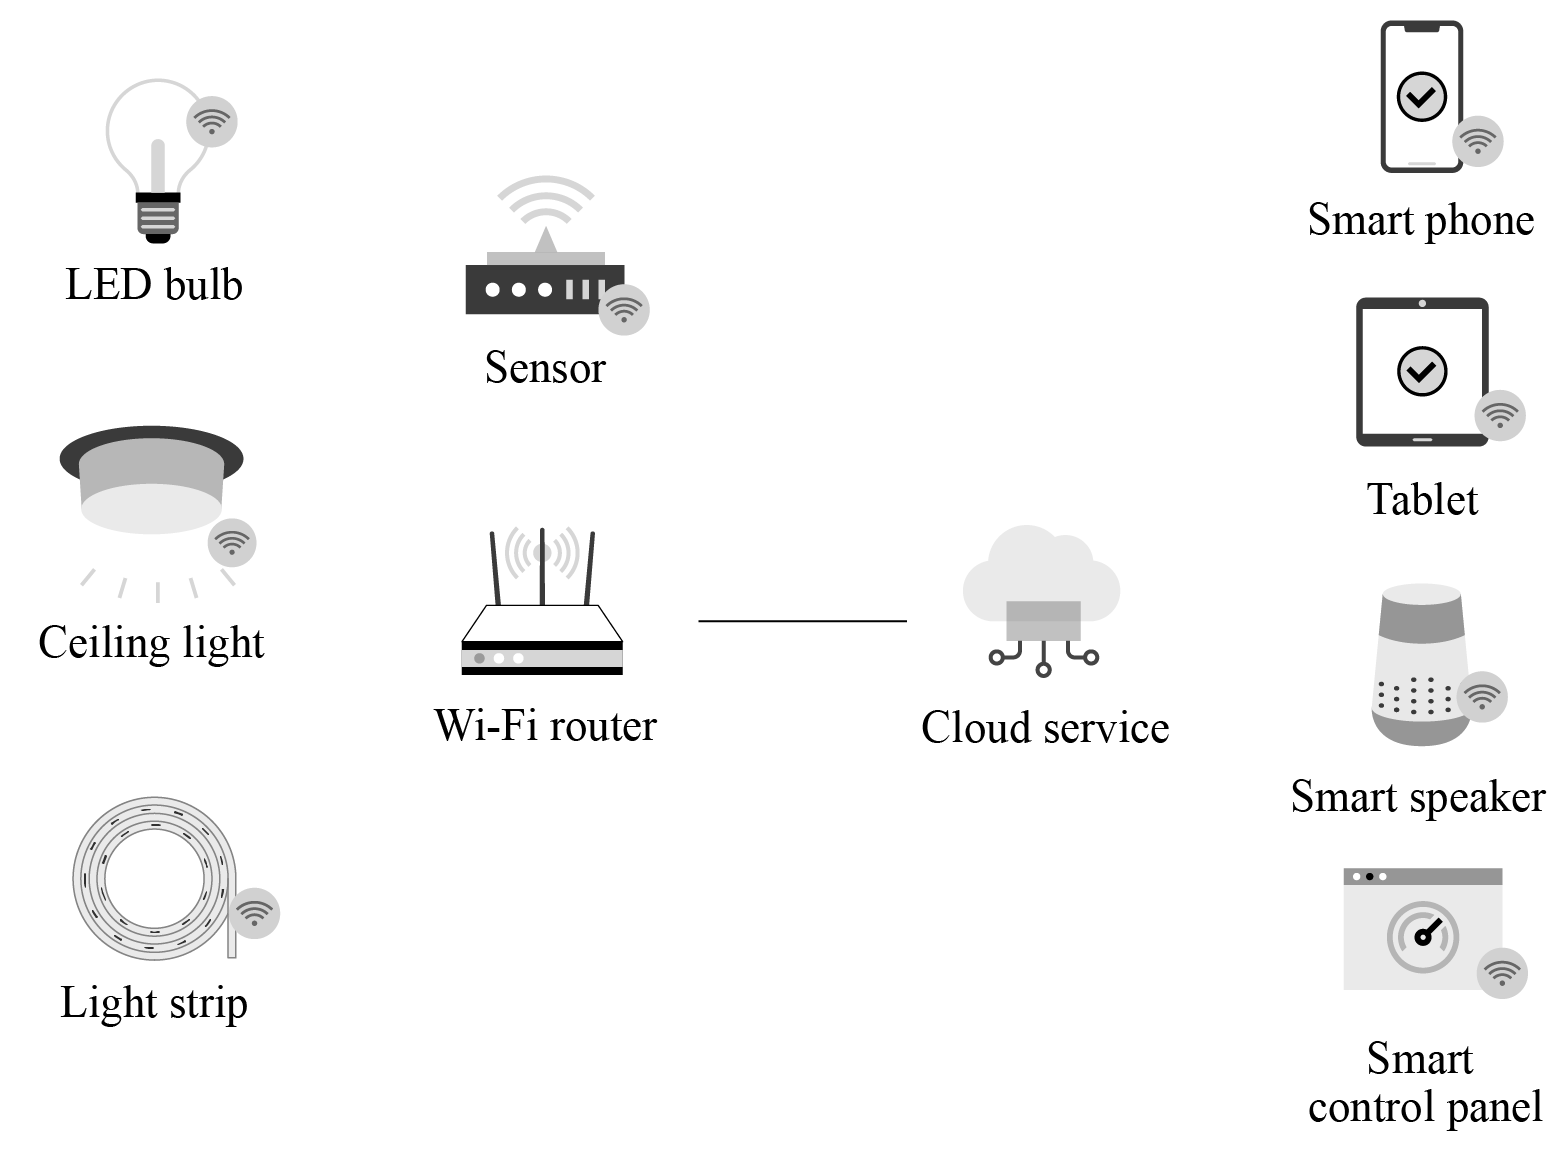
\includegraphics[width=0.6\textwidth]{D5Z/5-1}
    \caption{Structure of smart light system}
\end{figure}

From the description above, we can see that the main features of smart light products is to be controlled through wireless connection. Now we will take the colour-changing smart LED light as an example to explain the main components of smart light products and how to control them.

Figure 5.2 shows the structure of a smart LED bulb, including an E27 standard lamp holder, a plastic-wrapped aluminium lamp body, a power supply \& an LED driver board, a Wi-Fi module, LED beads \& an aluminium substrate, and a highly transparent lampshade. Compared with traditional LED bulbs, a smart LED bulb has an additional Wi-Fi module. So how does this Wi-Fi module help control the light wirelessly? The following sections will further elaborate on the functional implementation.

\begin{figure}[h!]
    \centering
    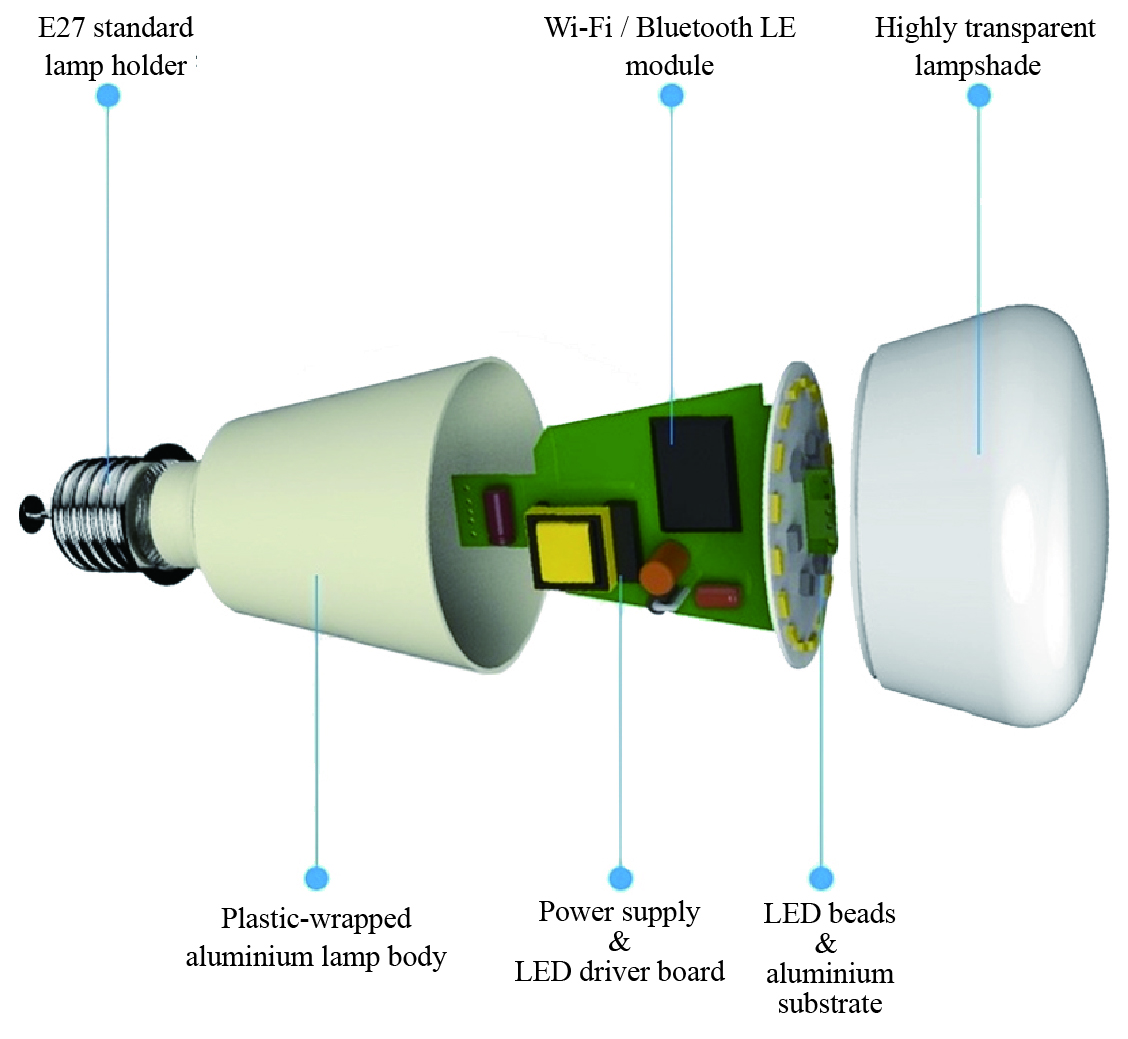
\includegraphics[width=0.55\textwidth]{D5Z/5-2}
    \caption{Structure of smart LED bulb}
\end{figure}

Figure 5.3 shows the functional block diagram of a smart LED bulb, which mainly includes a 220 V AC-DC power supply module, a constant-current LED driver, a 3.3 V output auxiliary power supply, a PWM control and wireless communication module, and LED beads of various colours.

\begin{figure}[h!]
    \centering
    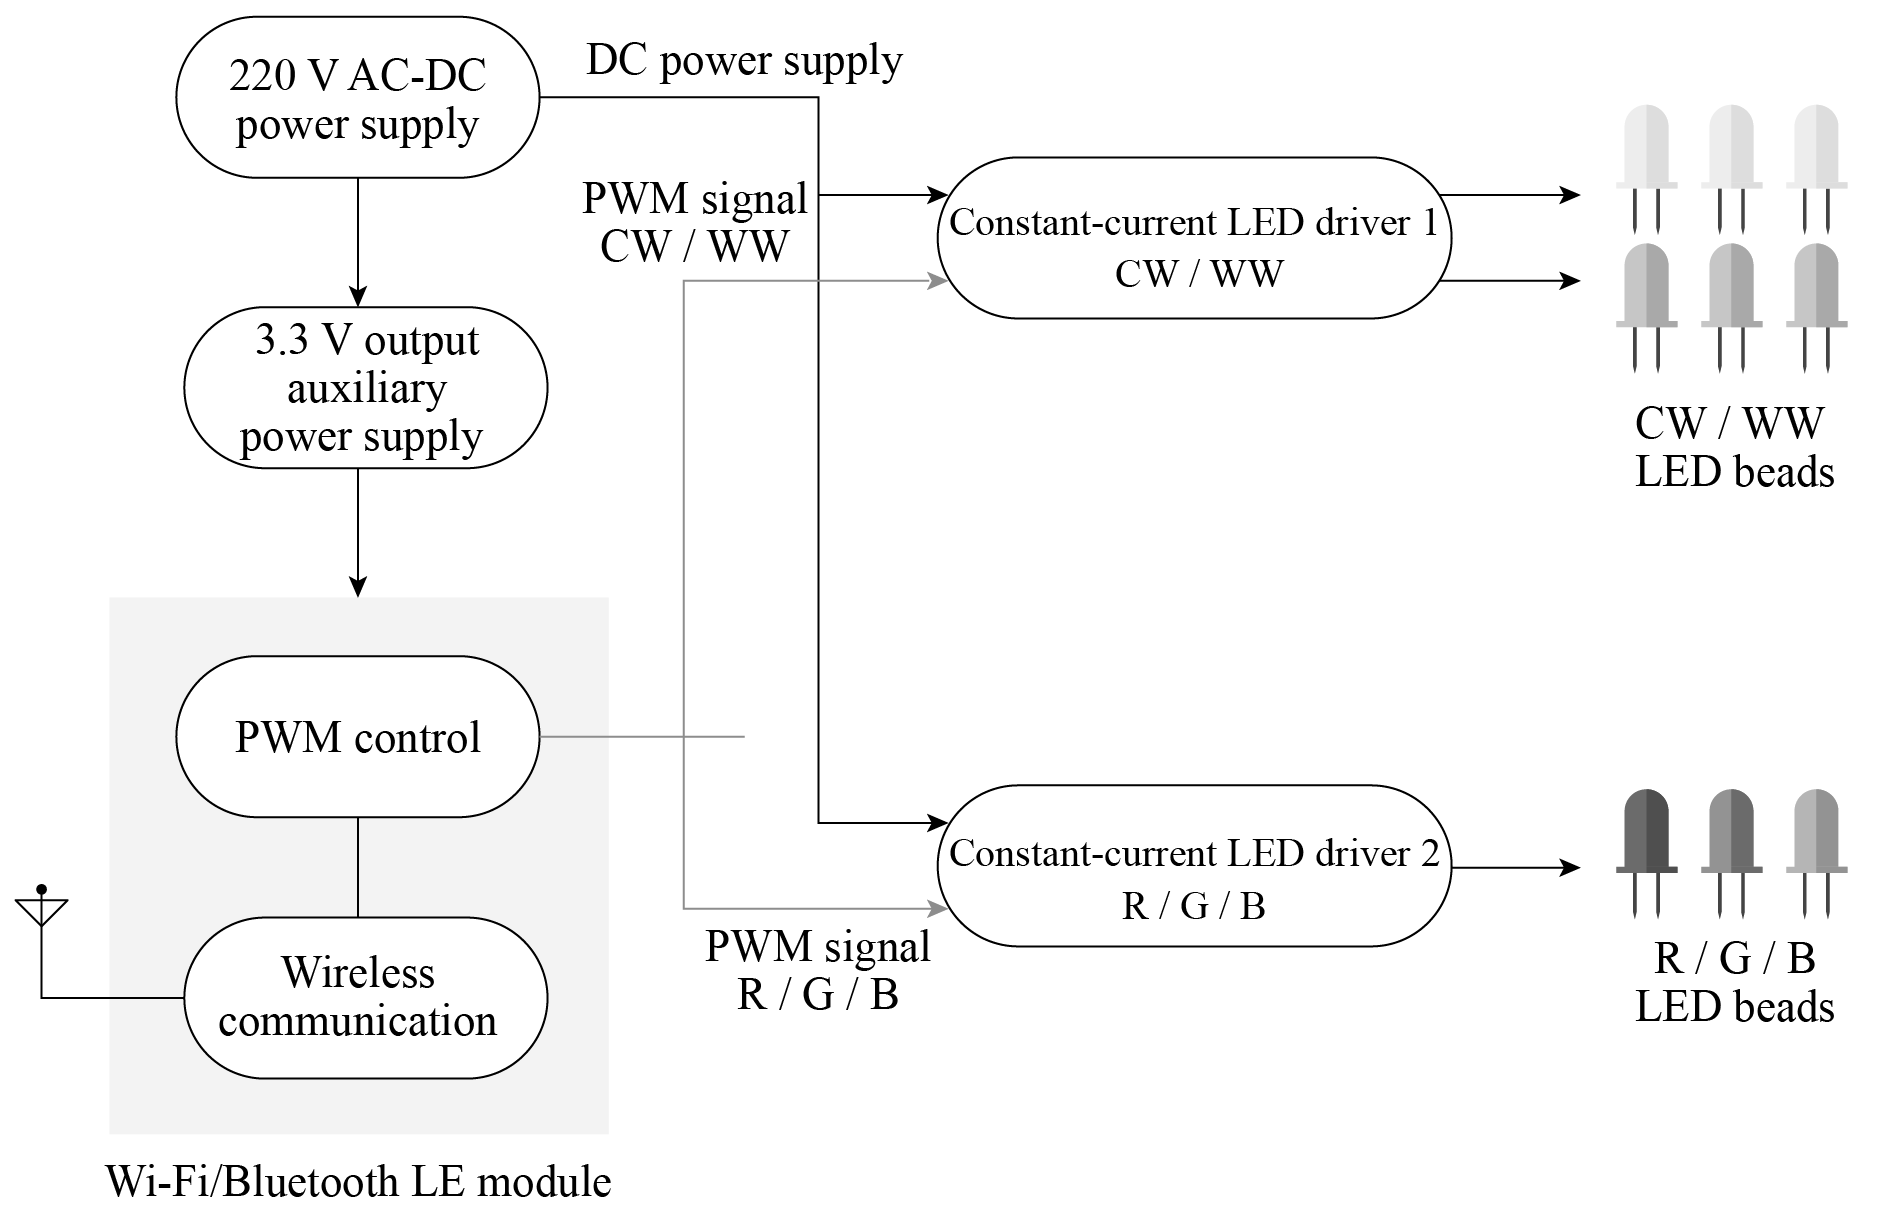
\includegraphics[width=0.7\textwidth]{D5Z/5-3}
    \caption{Block diagram of functional units for smart LED bulb}
\end{figure}

Before detailing each functional unit, let’s first take a glance at how they manage to change the brightness and colour of the lighting as a whole. The key lies in the LED lamp beads.

LED lamp beads can be dimmed in two ways: analogue dimming and digital dimming. Analogue dimming changes LED light output by simply adjusting the DC current in the circuit; while digital dimming, also known as PWM dimming, is achieved by varying the conduction time of forward current through turning on/off LEDs using PWM signals of different pulse widths. Section 6.3.3 will describe PWM dimming in detail. Here we will briefly introduce PWM dimming using PWM signals.

When using a controllable constant-current source to drive LED beads, to adjust colour temperature, you can change the duty cycles of PWM signals on two channels to adjust the current of warm-white (WW) and cool-white (CW) LED beads; to adjust light colours, you can change the duty cycles of PWM signals on three channels to adjust the brightness of corresponding colours so that the smart LED light emits the mixed colour of different lamp beads.

Knowing the basics of light dimming and colour change, now let’s dig into the functional units one by one.

\begin{term}{220 V AC-DC power supply}
    The input power of smart LED lights is usually high-voltage AC, and the standard household AC in China is 220 V. The 220 V AC-DC power module first converts the AC to DC through a rectifier bridge, and then reduces it to 18 $\sim$ 40 V for the constant-current LED drivers. Since the operating voltage of the PWM control and wireless communication module is 3.3 V, there is another auxiliary power supply to reduce the DC power to 3.3 V.
\end{term}

\begin{term}{Constant-current LED driver}
    To ensure consistency in the emission of multiple LED beads, you can use a series circuit and drive the LEDs with a constant current source. The brightness of the LEDs can be adjusted by controlling the constant current source using PWM signals. Constant-current LED driver 1 is used to drive the LEDs in cool white (CW) and warm white (WW), and the output power is relatively higher; constant-current LED driver 2 is used to drive red (R) / green (G) / blue (B) LEDs, mainly for changing colours, and the output power is lower.
\end{term}

\begin{term}{LED beads}
    In smart LED lights, there are usually warm-white, cool-white, red, green, and blue LED beads, among which more warm-white and cool-white beads are used for lighting, and less red, green or blue beads for colour adjustment.
\end{term}

\begin{term}{PWM control and wireless communication}
    In smart light products, to realise PWM control and wireless communication functions, a highly-integrated system-on-a-chip (SoC) is usually used. SoC supports multiple PWM signal outputs, as well as one or more mainstream wireless communication protocols such as Wi-Fi, Bluetooth LE, or ZigBee. It can run embedded RTOS, and supports software application development. With chips of Wi-Fi connectivity, you can connect your product to the Internet and cloud servers through a Wi-Fi router; with chips of Bluetooth LE or ZigBee functions, you need to configure a gateway device to connect to an Ethernet or Wi-Fi router first and then get it connected to the Internet and cloud servers.
\end{term}

The introduction above explains the main components of smart LED lights, as well as the realisation of dimming and colour change functions. It can be concluded that the biggest difference between smart light products and ordinary light products lies in the use of PWM control and wireless communication. The following sections of this chapter will focus on how to design the minimal hardware system based on the ESP32-C3 chip to realise PWM dimming, colour change, and wireless communication. The design is also applicable to other types of smart light products such as spotlights, ceiling lights, lamps, light strips, etc.

\section{Hardware Design of ESP32-C3 Core System}

Through Section 5.1, we can see that the PWM control and wireless communication module is the core unit of smart light products, which distinguishes them from traditional light products. Then how should we design this core system to implement the functions of smart light products? In this section, we’ll use the ESP32-C3 chip to demonstrate its hardware design.

ESP32-C3 is a highly-integrated SoC equipped with a 32-bit RISC-V processor, supporting 2.4 GHz Wi-Fi and Bluetooth LE connectivity. The functional block diagram of ESP32-C3 is shown in Figure 5.4.

\begin{figure}[h!]
    \centering
    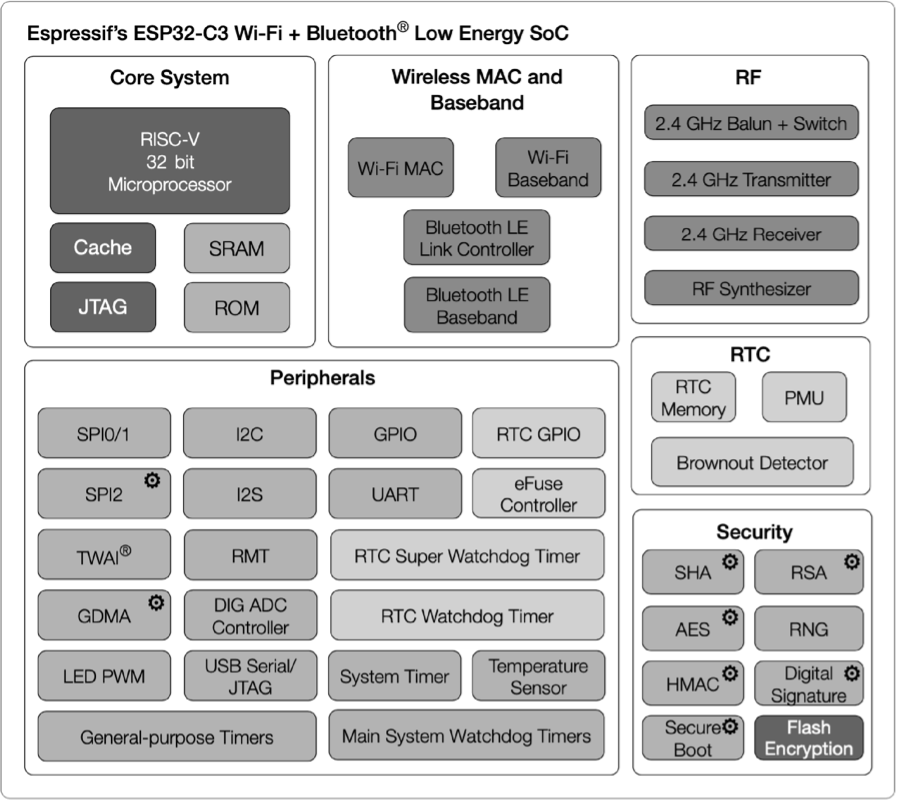
\includegraphics[width=0.65\textwidth]{D5Z/5-4}
    \caption{Block diagram of ESP32-C3 functions}
\end{figure}

ESP32-C3 has the following features:

\begin{itemize}
    \item A 32-bit RISC-V single-core processor with a four-stage pipeline which operates at up to 160 MHz.
    \item A \textbf{complete Wi-Fi subsystem} which complies with IEEE 802.11b/g/n protocol and supports Station mode, SoftAP mode, SoftAP + Station mode, and promiscuous mode.
    \item A \textbf{Bluetooth LE subsystem} which supports Bluetooth 5 and Bluetooth mesh.
    \item Storage capacities ensured by 400 KB SRAM and 384 KB ROM on the chip, and SPI, Dual SPI, Quad SPI, and QPI interfaces that allow connection to external flash.
    \item \textbf{Reliable security mechanisms} ensured by cryptographic hardware accelerators that support AES-128/256, Hash, RSA, HMAC, digital signature and secure boot, external memory encryption and decryption, random number generator, and permission control on accessing internal memory, external memory, and peripherals.
    \item \textbf{A rich set of peripheral interfaces} which are ideal for various scenarios and complex applications; \textbf{22 programmable GPIOs} that can be configured flexibly to support LED PWM, UART, I2C, SPI, I2S, ADC, TWAI, RMT, and USB Serial/JTAG applications.
\end{itemize}

The ESP32-C3 series of chips has several variants, including the version with in-package SPI flash. ESP8685 is a small package version of ESP32-C3, as shown in Table 5.1.


\begin{table}[h!]
    \renewcommand{\arraystretch}{1.2}
    \caption{ESP32-C3 series}
    \begin{tabular}{|>{\Centering}m{9em}|>{\Centering}m{9em}|>{\Centering}m{10em}|>{\Centering}m{10em}|}
        \hline
        \rowcolor{LightBlue} \textbf{MPN}&\textbf{Flash (MB)}&\textbf{Temp (℃)}&\textbf{Size (mm)}\\
        \hline
        ESP32-C3&—&--40 $\sim$ 105&QFN32 (5×5)\\
        \hline
        ESP32-C3-FN4&4&--40 $\sim$ 85&QFN32 (5×5)\\
        \hline
        ESP32-C3-FH4&4&--40 $\sim$ 105&QFN32 (5×5)\\
        \hline
        ESP32-C3-FH4AZ&4&--40 $\sim$ 105&QFN32 (5×5)\\
        \hline
        ESP8685H2&2&--40 $\sim$ 105&QFN32 (4×4)\\
        \hline
        ESP8685H4&4&--40 $\sim$ 105&QFN32 (4×4)\\
        \hline
    \end{tabular}
\end{table}

\note{\textbullet\ For ESP32-C3FH4AZ, ESP8685H2, and ESP8685H4, pins for flash connection are not bonded.

\textbullet\ Nomenclature of ESP32-C3 series: \textbf{F} stands for in-package flash, \textbf{H/N} indicates the flash temperature, and \textbf{AZ} is other identification code.}

The core circuit for ESP32-C3 requires about 20 resistors, capacitors, and inductors in total, as well as one crystal and one SPI flash. The high integration of ESP32-C3 makes it suitable for small-sized applications such as smart light products. Figure 5.5 and Figure 5.6 show the block diagram and the schematic of ESP32-C3 core circuit.

\begin{figure}[h!]
    \centering
    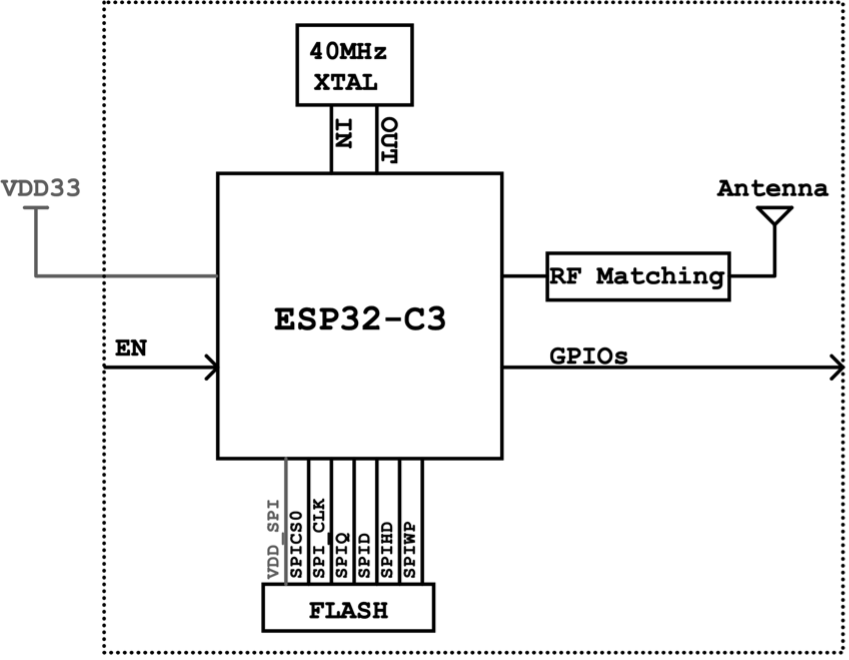
\includegraphics[width=0.55\textwidth]{D5Z/5-5}
    \caption{Block diagram of ESP32-C3 core circuit}
\end{figure}

The following explains in detail the schematics and PCB layout of ESP32-C3.

\begin{figure}[h!]
    \centering
    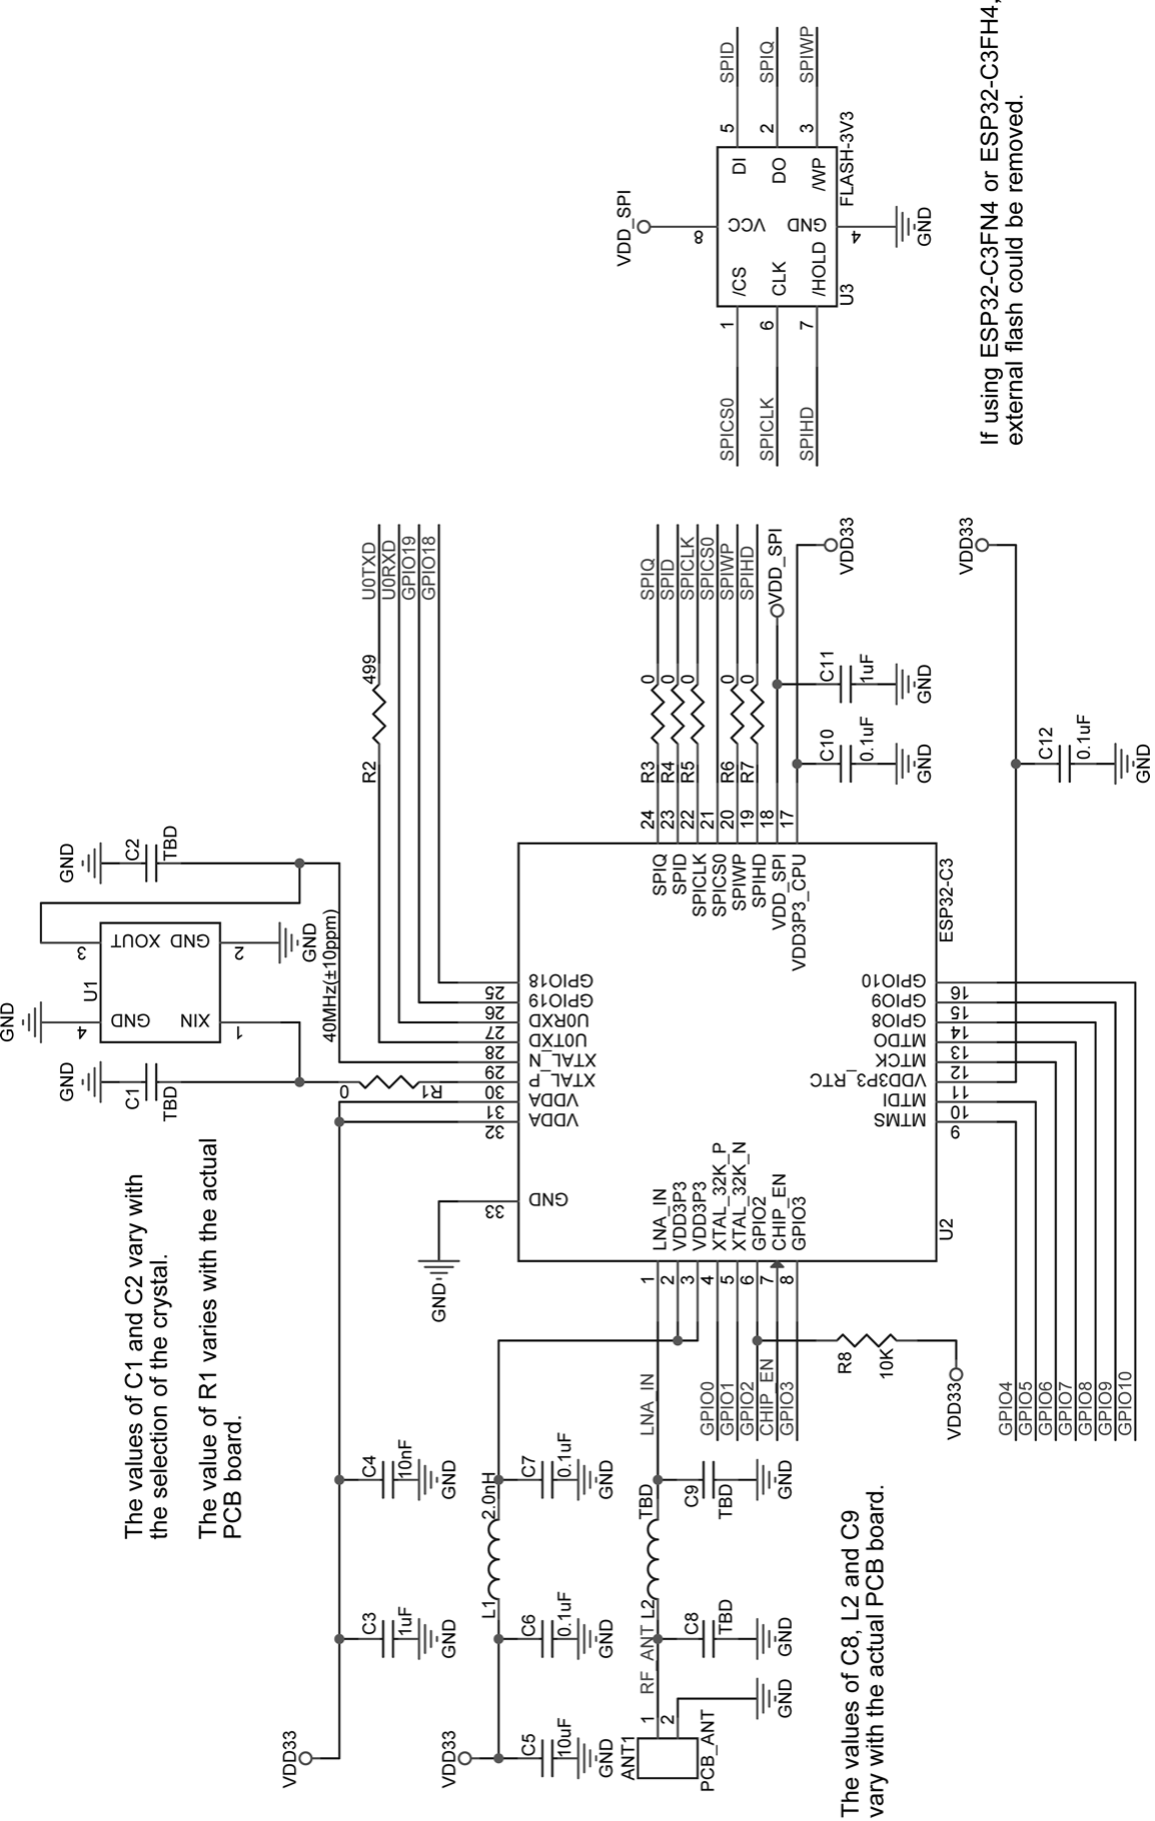
\includegraphics[width=0.83\textwidth]{D5Z/5-6}
    \caption{Schematic of ESP32-C3 core circuit}
\end{figure}

\subsection{Power Supply}
Pin 11 and pin 17 are the power supply pins for RTC IO and CPU IO respectively, in a voltage range of 3.0 V $\sim$ 3.6 V. We recommend adding a 0.1 $\mu$F capacitor close to each power supply pin. When working as an output power supply pin, VDD\_SPI (pin 18) mainly powers external SPI flash. We recommend adding a 1 $\mu$F filter capacitor between VDD\_SPI and ground. When VDD\_SPI works as the power supply pin for in-package flash or external 3.3 V flash, the voltage of VDD3P3\_CPU should be maintained at 3.0 V or above, to ensure the flash’s operation.

Pin 2, pin 3, pin 31, and pin 32 are the analogue power supply pins, working at 3.0 V $\sim$ 3.6 V. Please note that when ESP32-C3 works in transmission (TX) mode, the instantaneous current will be higher and may cause power rail collapse. Therefore, it is highly recommended to add a 10 $\mu$F capacitor to the power trace, which can work in conjunction with the 0.1 $\mu$F capacitor. In addition, an LC filter circuit needs to be added near pin 2 and pin 3 to suppress high-frequency harmonics. The inductor’s rated current is preferably 500 mA or above. Refer to the core circuit schematic and place the appropriate decoupling capacitor near each analogue power pin.

For a single power supply, the recommended voltage is 3.3 V, and the recommended output current is 500 mA or above. We also suggest adding an ESD protection diode at the power entrance.

\subsection{Power-on Sequence and System Reset}
ESP32-C3 uses a 3.3 V system power supply. The chip should be activated after the power rails have stabilised. This is achieved by delaying the activation of pin 7 CHIP\_EN after the 3.3 V rails have been brought up. Figure 5.7 shows the power-up and reset timing of ESP32-C3. Details about the parameters are listed in Table 5.2.

\begin{figure}[h!]
    \centering
    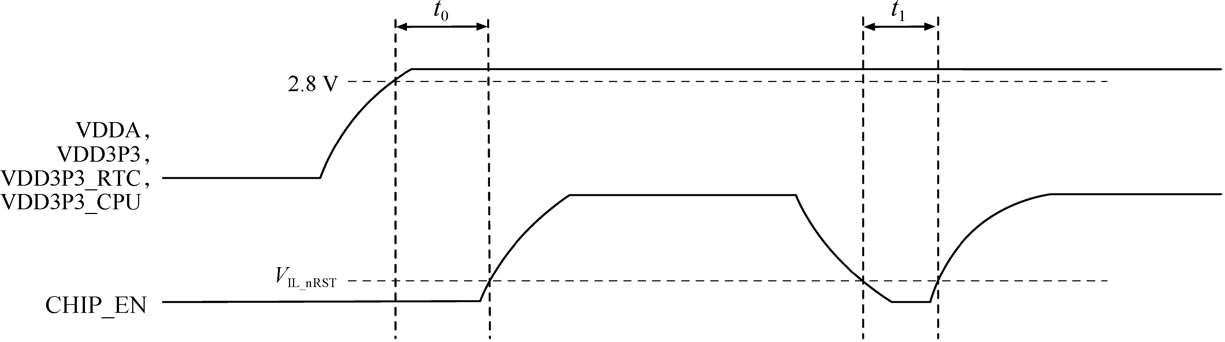
\includegraphics[width=\textwidth]{D5Z/5-7}
    \caption{ESP32-C3 power-up and reset timing}
\end{figure}

\begin{table}[h!]
    \renewcommand{\arraystretch}{1.4}
    \caption{Parameter description of ESP32-C3 power-up and reset timing}
    \begin{tabular}{|>{\Centering}m{5em}|m{29em}|>{\Centering}m{4em}|}
        \hline
        \rowcolor{LightBlue} \textbf{Parameter}&\multicolumn{1}{c|}{\textbf{Description}}&\textbf{Min.}\\
        \hline
        \textit{t$_0$}&Time between bringing up the VDDA, VDD3P3, VDD3P3\_RTC, and VDD3P3\_CPU rails, and activating CHIP\_EN&50 $\mu$s\\
        \hline
        \textit{t$_1$}&Duration of CHIP\_EN signal level $< V_{IL\_nRST}$ to reset the chip&50 $\mu$s\\
        \hline
    \end{tabular}
\end{table}

To ensure that the power supply to ESP32-C3 is stable during power-up, it is advised to add an RC delay circuit at the CHIP\_EN pin. The recommended setting for the RC delay circuit is usually $R = 10 k\Omega$ and $C = 1 \mu F$, while specific parameters should be adjusted based on the power-up timing of the power supply and the power-up and reset sequence timing of the chip.

CHIP\_EN can also be used as the reset pin of ESP32-C3. When CHIP\_EN is at low level, the reset voltage (V$_{IL\_nRST}$) should be (--0.3 $\sim$ 0.25) × $V_{DD}$ (where $V_{DD}$ is the I/O voltage for a particular power domain of pins). To avoid reboots caused by external interference, route the CHIP\_EN trace as short as possible, and add a pull-up resistor as well as a capacitor to ground. Note that CHIP\_EN pin must not be left floating.

\subsection{SPI Flash}
ESP32-C3 supports external flash of up to 16 MB, which is mainly used for storing program firmware, system parameters, user parameters, user data, etc. The SPI flash is powered by VDD\_SPI. We recommend reserving a serial resistor (initially of 0 $\Omega$) on the SPI line, to lower the driving current, adjust timing, reduce crosstalk and external interference, etc. ESP32-C3FH4/FN4 has an in-package 4 MB SPI flash.

\subsection{Clock Source}
Currently, the ESP32-C3 firmware supports 40 MHz crystal. The specific capacitance of C1 and C2 depends on further testing of, and adjustment to, the overall performance of the whole circuit. Please add a component (i.e., R1 in Figure 5.6) in series on the XTAL\_P clock trace to minimise the impact of crystal harmonics on RF performance. The value of this component (initially of 24 nH) depends on further RF testing. Note that the accuracy of the selected crystal needs to be ±10 ppm. In actual use, as the temperature of smart light products rises, the frequency deviation of the crystal will also increase. Therefore, please ensure that the frequency deviation of the crystal does not exceed 25 ppm, so as not to affect Wi-Fi communication.

Although ESP32-C3 has integrated an RC oscillator as the RTC clock source, it also supports an external 32.768 kHz crystal to act as the RTC clock source. Figure 5.8 shows the schematic of the external 32.768 kHz crystal.

\begin{figure}[h!]
    \centering
    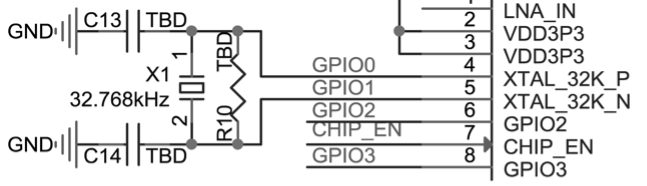
\includegraphics[width=0.7\textwidth]{D5Z/5-8}
    \caption{Schematic of ESP32-C3’s external crystal (RTC)}
\end{figure}

\note{
\textbullet\ Requirements for the 32.768 kHz crystal: 

\leftskip 2em
- Equivalent series resistance (ESR) $\leq$ 70 k$\Omega$.

- Load capacitance at both ends should be configured according to the crystal’s specification.

\leftskip 1em
\textbullet\ The parallel resistor R10 is used for biasing the crystal circuit ($5 M\Omega < R10 \leq 10 M\Omega$). In general, you do not need to populate R10.

\textbullet\ If the RTC source is not required, then pin 4 (XTAL\_32K\_P) and pin 5 (XTAL\_32K\_N) can be used as normal GPIOs.}

\subsection{RF and Antenna}
In your circuit design, please add a $\pi$-matching network between the RF port (LNA\_IN) and the antenna, for antenna matching purpose. A CLC network is preferred, as shown in Figure 5.9. The parameters of C8, L2, and C9 in the matching network are subject to the actual antenna and PCB layout.

\begin{figure}[h!]
    \centering
    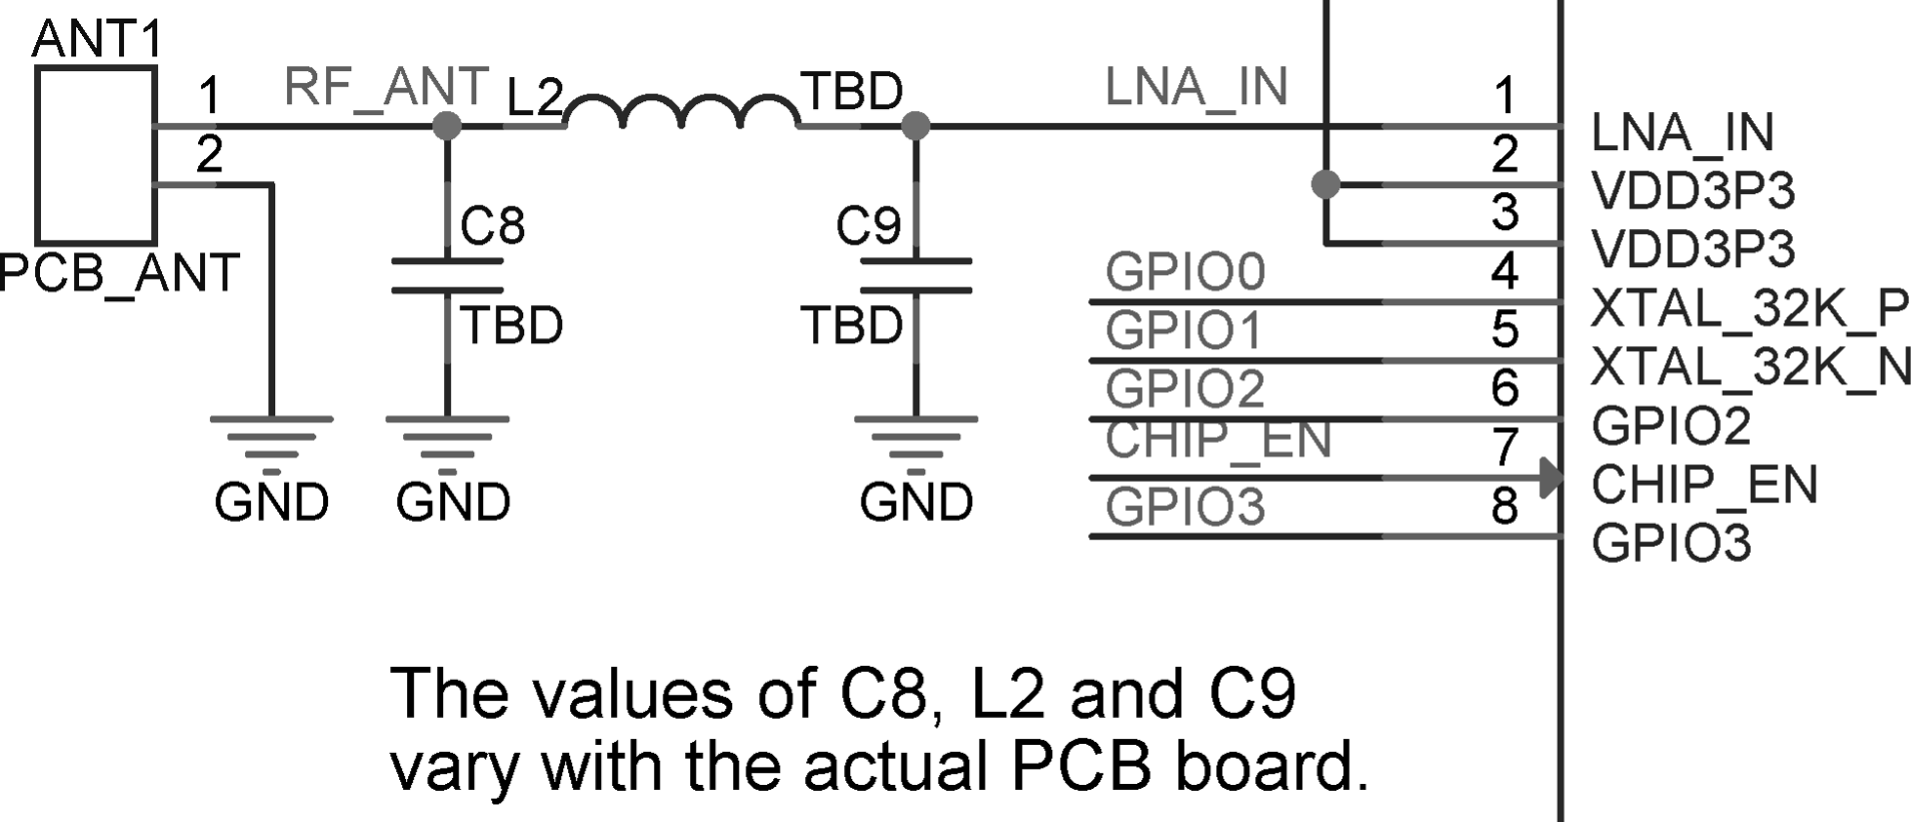
\includegraphics[width=0.7\textwidth]{D5Z/5-9}
    \caption{CLC circuit for ESP32-C3 RF matching}
\end{figure}

The antenna can be selected based on product design and the overall cost. You can choose PCB onboard antenna, or an external antenna such as rod antenna, FPC antenna, ceramic antenna, 3D metal antenna, etc. Commonly-used antenna types are shown in Figure 5.10. Their installation methods and characteristics are provided in Table 5.3.

\begin{figure}[h!]
    \centering
    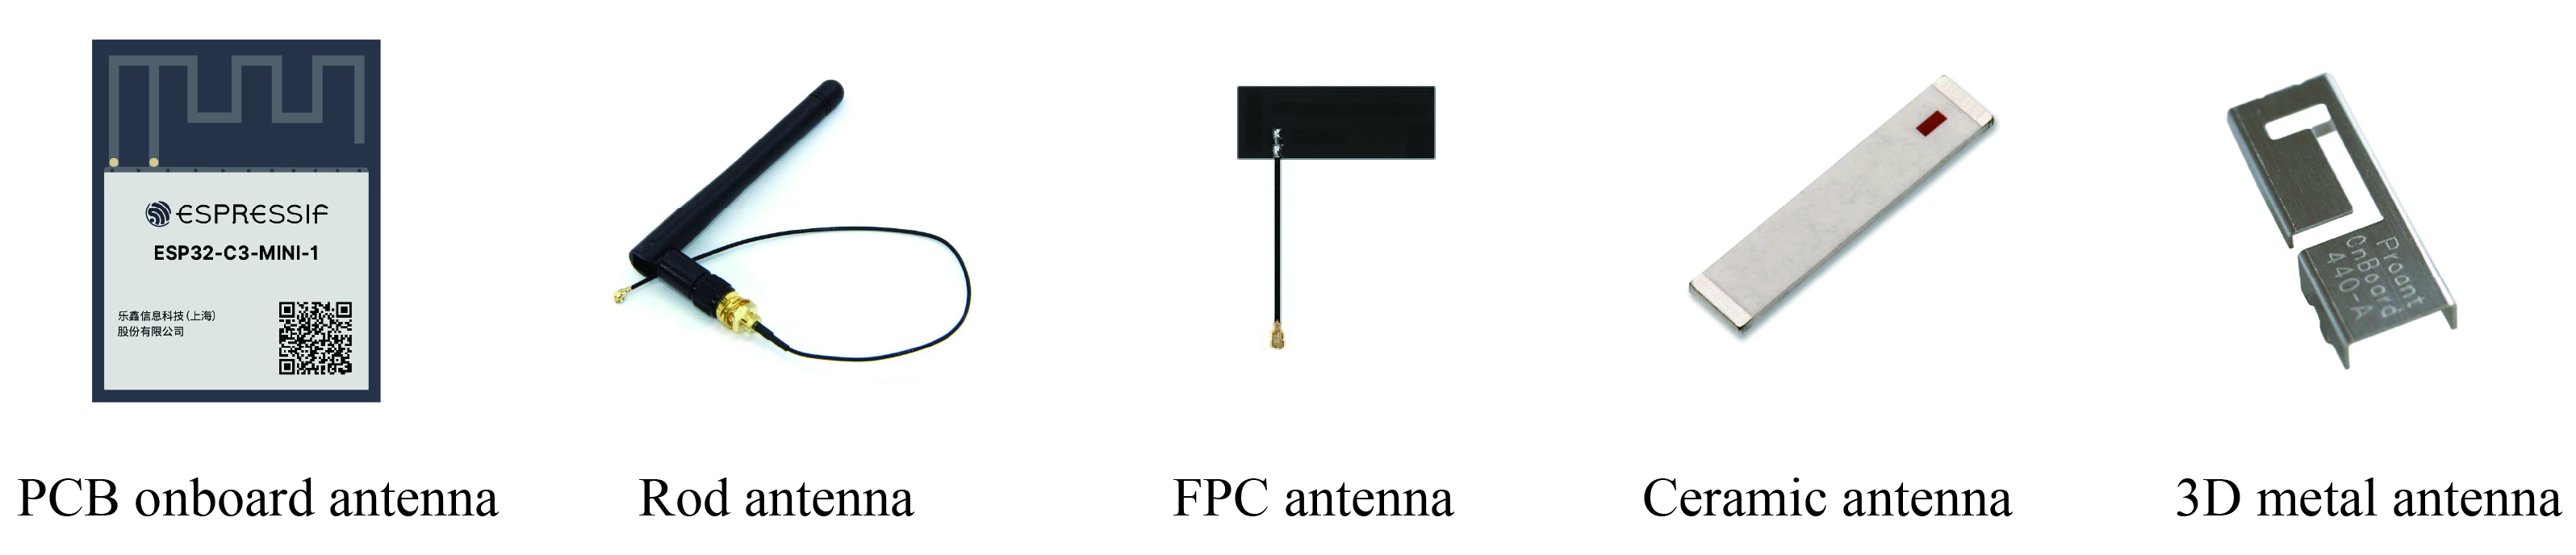
\includegraphics[width=0.9\textwidth]{D5Z/5-10}
    \caption{Commonly-used antenna types}
\end{figure}

\begin{table}[h!]
    \renewcommand{\arraystretch}{1.2}
    \caption{Installation methods and characteristics of commonly-used antenna types}
    \begin{tabular}{|>{\Centering}m{8em}|>{\Centering}m{10em}|>{\RaggedRight}m{20.5em}|}
        \hline
        \rowcolor{LightBlue} \textbf{Antenna Type}&\textbf{Installation Methods}&\multicolumn{1}{c|}{\textbf{Characteristics}}\\
        \hline
        PCB\newline onboard antenna&PCB onboard&Low cost, medium gain, usually integrated on modules\\
        \hline
        Rod antenna&External connection\newline through I-PEX connector&High cost, high gain, less susceptible to interference, good omni-directional performance\\
        \hline
        FPC antenna&Adhesive installation&Medium cost, medium gain, can be adhered to the package, suitable for products with restricted structure\\
        \hline
        Ceramic antenna&PCB mounting&Medium cost, low gain, small size, suitable for small-sized modules\\
        \hline
        3D metal antenna&PCB mounting&High cost, high gain, less susceptible to interference, good omni-directional performance\\
        \hline
    \end{tabular}
\end{table}

The RF performance can be optimised through antenna matching. After matching, you can use CMW500, WT-200, IQ View, IQ Xel or other comprehensive RF testers to test RF performance of the ESP32-C3 core board. RF test includes conducted test and radiatied test.

\begin{term}{Conducted test}
    In conducted tests, use a 50 $\Omega$ RF cable to connect the RF output port of the ESP32-C3 core board to the tester’s RF port, and run the RF test software on the PC. Through the software, you can communicate with the ESP32-C3 core board and the tester, thus controlling the test. The conducted test set-up is shown in Figure 5.11.

    \begin{figure}[h!]
        \centering
        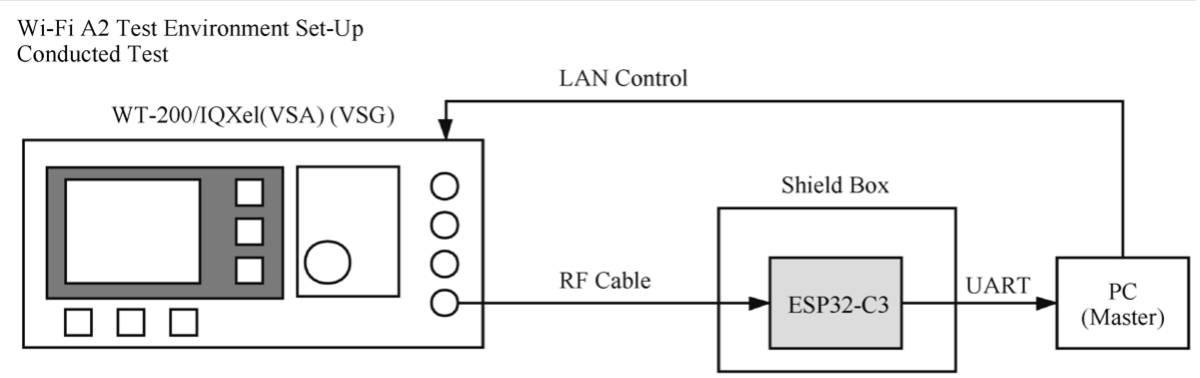
\includegraphics[width=\textwidth]{D5Z/5-11}
        \caption{Conducted test set-up for ESP32-C3 core board}
    \end{figure}
\end{term}

\begin{term}{Radiated test}
    When performing a radiated test, place the tester’s antenna and ESP32-C3 board’s antenna close to each other in the shield box. It is recommended that the distance between the two antennas be about 10 cm. Control the test through PC software. The radiated test set-up is shown in Figure 5.12.

    \begin{figure}[h!]
        \centering
        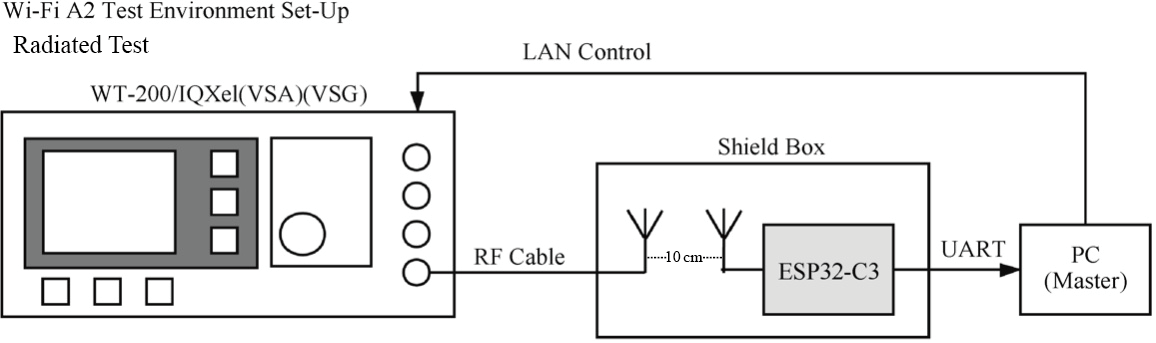
\includegraphics[width=\textwidth]{D5Z/5-12}
        \caption{Radiated test set-up for ESP32-C3 core board}
    \end{figure}
\end{term}

For Wi-Fi RF performance test, the primary test parameters are target transmit power, EVM, receiver sensitivity, and frequency error, as shown in Table 5.4.

\begin{table}[h!]
    \renewcommand{\arraystretch}{1.5}
    \caption{Key parameters for Wi-Fi RF test}
    \begin{tabular}{|>{\Centering}m{12.5em}|>{\Centering}m{6.5em}|>{\Centering}m{5em}|>{\Centering}m{7em}|>{\Centering}m{6.5em}|}
        \hline
        \rowcolor{LightBlue} \textbf{Working Mode and Rate}&\textbf{Target TX Power (dBm)}&\textbf{EVM (dB)}&\textbf{Receiver Sensitivity (dBm)}&\textbf{Frequency Error (ppm)}\\
        \hline
        IEEE 802.11b, 1 Mbit/s&21.0±2.0&$<-$24.5&$<-$98&±25\\
        \hline
        IEEE 802.11g, 54 Mbit/s&19.0±2.0&$<-$27.5&$<-$76.2&±20\\
        \hline
        IEEE 802.11n, MCS7 HT20&18.5±2.0&$<-$29&$<-$74.4&±20\\
        \hline
        IEEE 802.11n, MCS7 HT40&18.5±2.0&$<-$28&$<-$71.2&±20\\
        \hline
    \end{tabular}
\end{table}

Figure 5.13 shows the spectral mask requirements in different working modes.

\begin{figure}[h!]
    \centering
    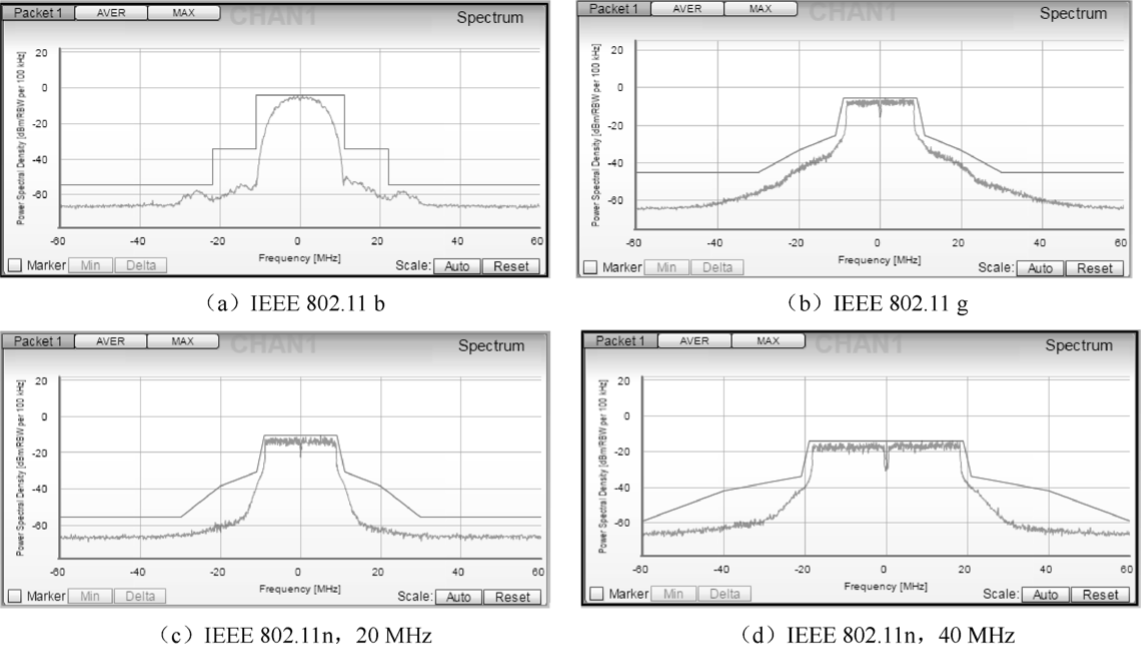
\includegraphics[width=0.9\textwidth]{D5Z/5-13}
    \caption{Spectral mask requirements in different working modes}
\end{figure}

\subsection{Strapping Pins}
ESP32-C3 has three strapping pins: GPIO2, GPIO8, and GPIO9. During the chip’s system reset, the strapping pins sample their voltage levels and store them into the latch until the chip is powered down or shut down. Depending on the stored voltage levels, the chip will enter different boot modes after system reset. The correspondence between the voltage levels and the boot modes is shown in Table 5.5. After reset, the strapping pins function as normal pins.

\begin{table}[h!]
    \renewcommand{\arraystretch}{1.2}
    \caption{Voltage level of strapping pins and corresponding boot mode}
    \begin{tabular}{|>{\Centering}m{8em}|>{\Centering}m{10em}|>{\Centering}m{10em}|>{\Centering}m{10em}|}
        \hline
        \rowcolor{LightBlue} \textbf{Strapping Pins}&\textbf{Default}&\textbf{SPI Boot}&\textbf{Download Boot}\\
        \hline
        GPIO2&N/A&1&1\\
        \hline
        GPIO8&N/A&Irrelevant&1\\
        \hline
        GPIO9&Weak internal pull-up&1&0\\
        \hline
    \end{tabular}
\end{table}

\subsection{GPIO and PWM Controller}
ESP32-C3 has 22 GPIO pins which can be assigned various functions by configuring corresponding registers. All GPIOs can be configured with internal pull-up, pull-down, or set to high impedance. GPIO MUX and GPIO Matrix are used to collectively control the GPIO pin signals of the chip. By utilising GPIO MUX and GPIO Matrix (as shown in Figure 5.14), it is possible to configure the peripheral input signals from any GPIO pin, and the peripheral output signals can also be connected to any GPIO pin.

\begin{figure}[h!]
    \centering
    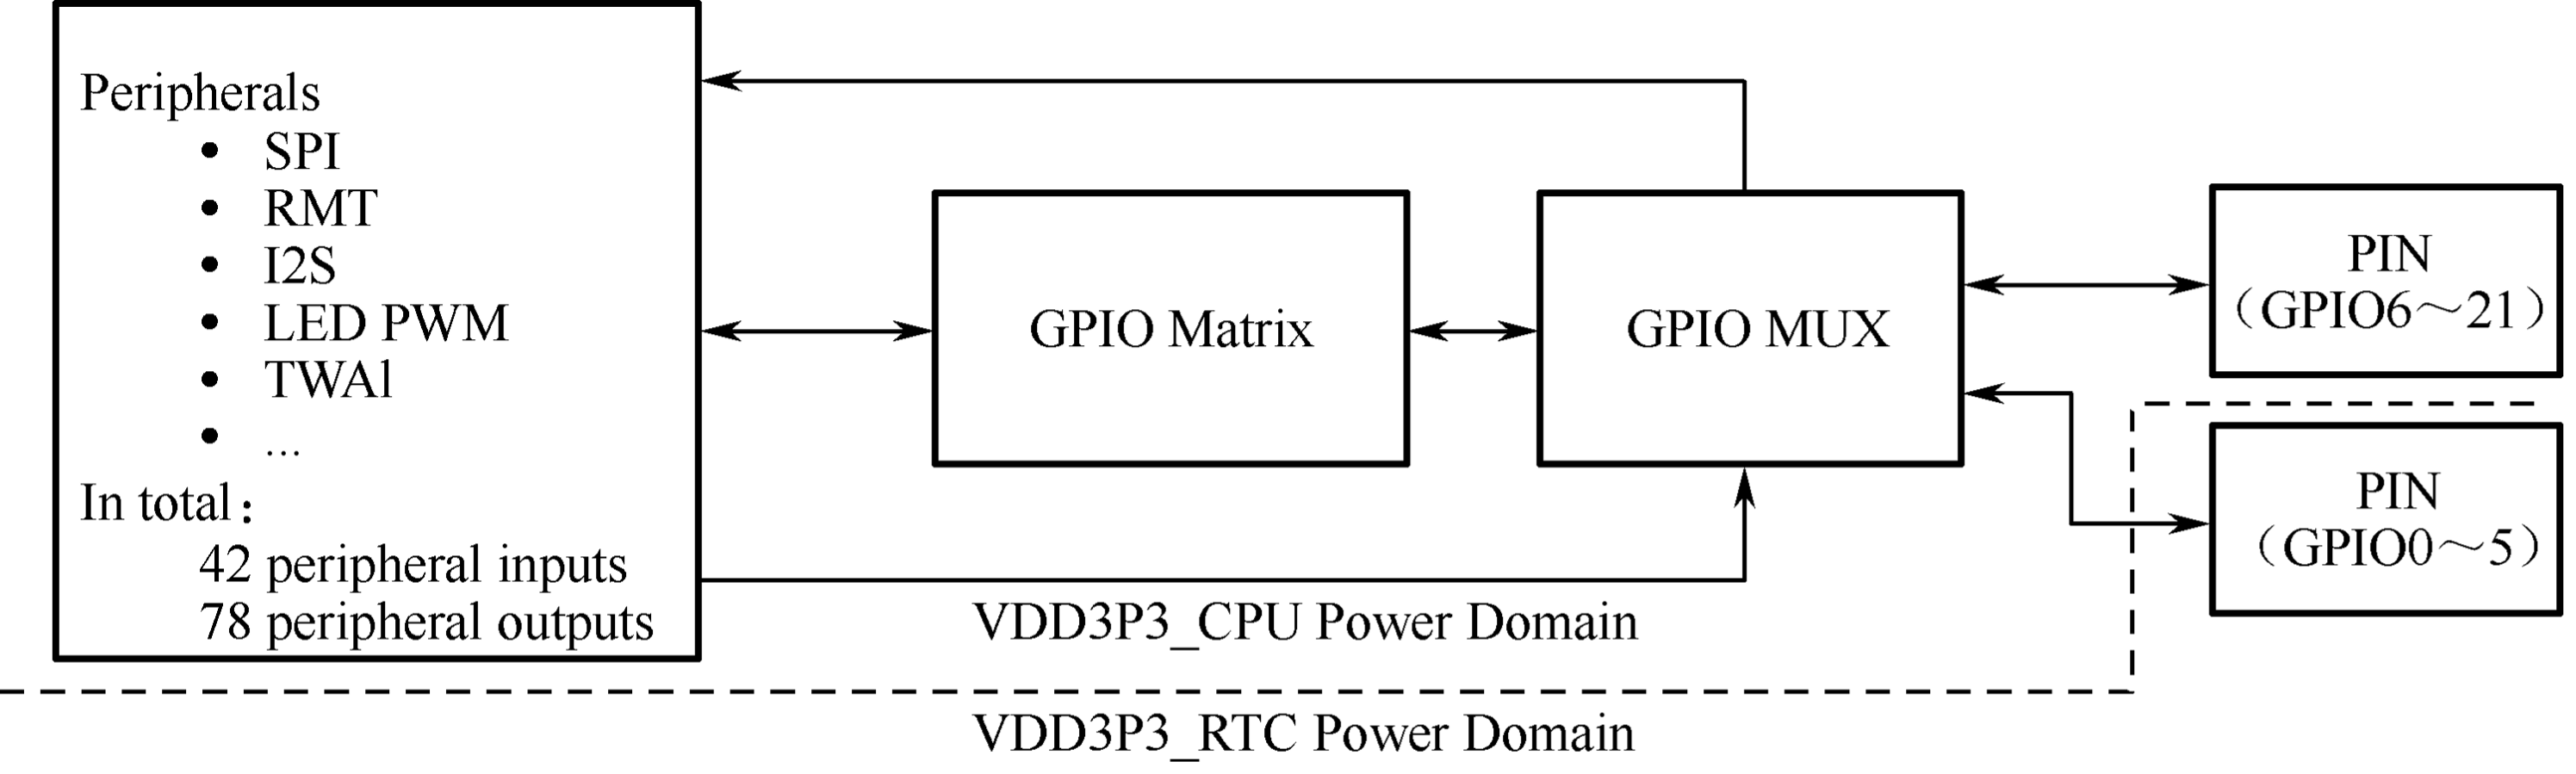
\includegraphics[width=0.9\textwidth]{D5Z/5-14}
    \caption{IO MUX and GPIO matrix}
\end{figure}

The PWM controller can generate independent PWM signals on six channels, which can be configured to any GPIO pins through the GPIO Matrix.

\section{Practice: Building a Smart Light System with ESP32-C3}
Section 5.2 introduced how to design the minimum hardware system (core circuit) and communication system for smart light products based on ESP32-C3. This minimum hardware system includes the main peripheral components and the antenna part which needs to be matched with the network analyser and RF tester according to the selected antenna type and the design of RF circuit. Antenna matching may be difficult for users who are new to RF. So, is there a ready-made minimum hardware system which has been tuned for RF performance, for users to get started quickly to develop a smart light product?

Yes, there ARE hardware modules based on the ESP32-C3 chip ready for operation. Apart from the chip, these modules also integrate a crystal oscillator, flash, antenna, RF circuit and main peripheral components. In addition, the modules have passed certification of SRRC, CE, FCC, and KCC, and can be directly applied to smart light products. In the following sections, we will choose one of the ESP32-C3 modules for smart light products design.

\subsection{Selecting Modules}
As shown in Table 5.6, in terms of the type of antenna, ESP32-C3 modules can be divided into PCB antenna modules and IPEX external antenna modules; in terms of size and pins, they can be divided into WROOM series and MINI series. Each module has two temperature range versions: --40 $\sim$ 85 ℃ version and --40 $\sim$ 105 ℃ version, suitable for smart lights of different temperature requirements. For lighting products such as LED bulbs which characterise high internal temperature, it is recommended to use the --40 $\sim$ 105 ℃ module. For other lighting products which do not have high internal temperature, the --40 $\sim$ 85 ℃ module is suitable.

\begin{table}[h!]
    \renewcommand{\arraystretch}{1.4}
    \caption{ESP32-C3 modules}
    \begin{tabular}{|>{\Centering}m{11em}|>{\Centering}m{11em}|>{\Centering}m{8em}|>{\Centering}m{8em}|}
        \hline
        \rowcolor{LightBlue} \textbf{Module}&\textbf{Antenna}&\textbf{Temp (℃)}&\textbf{Size (mm)}\\
        \hline
        \textbf{ESP32-C3-WROOM-02}\newline\vspace{6pt}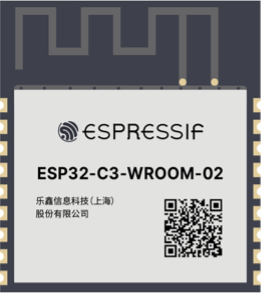
\includegraphics[width=0.21\textwidth]{D5Z/02}&PCB antenna&--40 $\sim$ 85 ℃/\newline--40 $\sim$ 105 ℃&18×20×3.2\\
        \hline
        \textbf{ESP32-C3-WROOM-02U}\newline\vspace{6pt}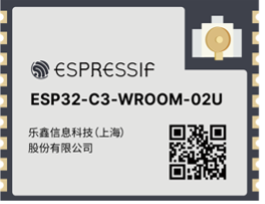
\includegraphics[width=0.21\textwidth]{D5Z/02U}&IPEX external antenna&--40 $\sim$ 85 ℃/\newline--40 $\sim$ 105 ℃&18×14.3×3.2\\
        \hline
        \textbf{ESP32-C3-MINI-1}\newline\vspace{6pt}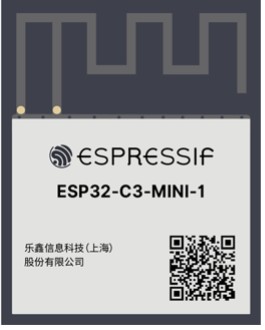
\includegraphics[width=0.21\textwidth]{D5Z/1}&PCB antenna&--40 $\sim$ 85 ℃/\newline--40 $\sim$ 105 ℃&13.2×16.6×2.4\\
        \hline
       \textbf{ ESP32-C3-MINI-1U}\newline\vspace{6pt}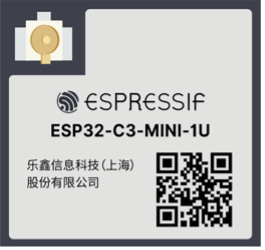
\includegraphics[width=0.21\textwidth]{D5Z/1U}&IPEX external antenna&--40 $\sim$ 85 ℃/\newline--40 $\sim$ 105 ℃&13.2×12.5×2.4\\
        \hline
    \end{tabular}
\end{table}

\note{You can also select one module from ESP8685-WROOM-01 to ESP8685-WROOM-07 series for a smaller package. For more information, please visit \href{https://products.espressif.com/\#/}{products.espressif.com}.}

\subsection{Configuring GPIOs of PWM Signals}
The PWM controller of ESP32-C3 can generate independent PWM signals on six channels, which can be assigned to any GPIOs through the GPIO matrix. In our design, five channels of PWM signals are used to control R (red), G (green), B (blue), CW (cool white), and WW (warm white) signals. In real application, we can use one channel to control the duty cycles of WW and CW LEDs to adjust the colour temperature, and another channel to control the total current to adjust the brightness of WW and CW LEDs. The GPIO configuration of each PWM signal is shown in Table 5.7.

\begin{table}[h!]
    \renewcommand{\arraystretch}{1.4}
    \caption{GPIO configuration for PWM signals}
    \begin{tabular}{|>{\Centering}m{0.48\textwidth}|>{\Centering}m{0.5\textwidth}|}
        \hline
        \rowcolor{LightBlue} \textbf{Function}&\textbf{GPIO Configuration}\\
        \hline
        R (Red)&GPIO3\\
        \hline
        G (Green)&GPIO4\\
        \hline
        B (Blue)&GPIO5\\
        \hline
        CW (Cool white)&GPIO7\\
        \hline
        WW (Warm white)&GPIO10\\
        \hline
    \end{tabular}
\end{table}

When selecting GPIOs, make sure that they are not at high level after chip start-up, otherwise the LED bulb may flicker when powered on. If no suitable GPIO is available, add a 10 k$\Omega$ pull-down resistor to the GPIO to prevent flickering. Any GPIOs on ESP32-C3 can be used for PWM function, as long as they are configured during initialisation after chip power-up.

Figure 5.15 shows the minimum control system based on the ESP32-C3-WROOM-02 module, which is connected to five LEDs of red, green, blue, cool white, and warm white.

\begin{figure}[h!]
    \centering
    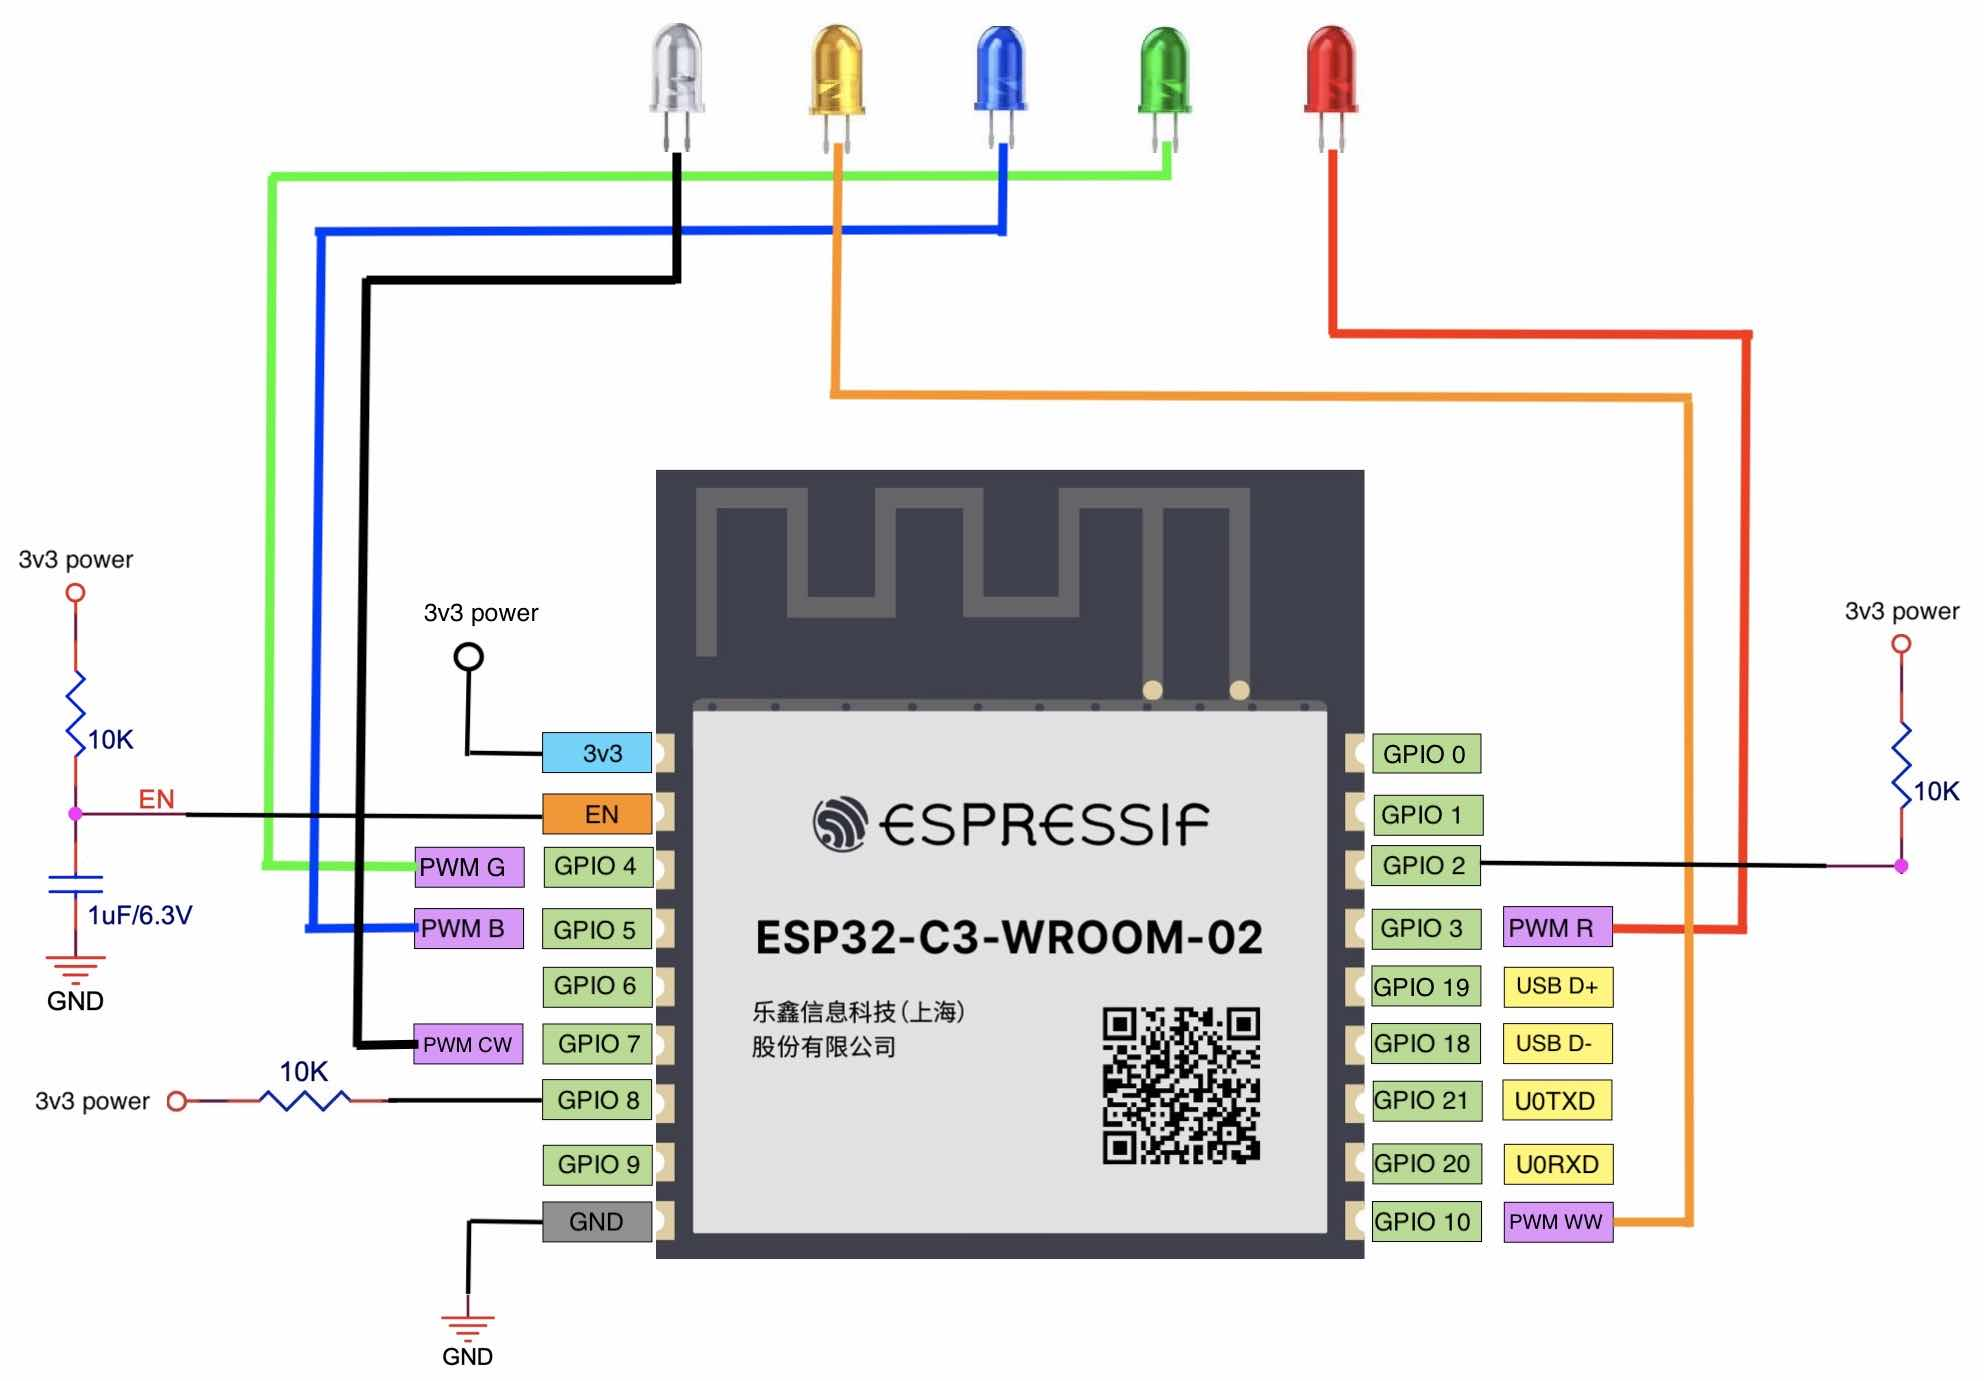
\includegraphics[width=0.9\textwidth]{D5Z/5-15}
    \caption{Minimum control system based on ESP32-C3-WROOM-02}
\end{figure}

\subsection{Downloading Firmware and Debugging Interface}
\subsubsection{1. Connect ESP32-C3 to a PC.}
The ESP32-C3 chip integrates a USB Serial/JTAG controller which makes external USB-to-UART bridge or JTAG adapter unnecessary. The USB on ESP32-C3 uses GPIO19 as D+ and GPIO18 as D--, and can be directly connected to the USB interface on the PC, so as to realise firmware download, log printing, and JTAG debugging. Figure 5.16 shows that an ESP32-C3 board is connected to a PC through the built-in USB Serial/JTAG controller. You may visit \url{https://bookc3.espressif.com/usb} for more applications of the USB Serial/JTAG controller.

\begin{figure}[h!]
    \centering
    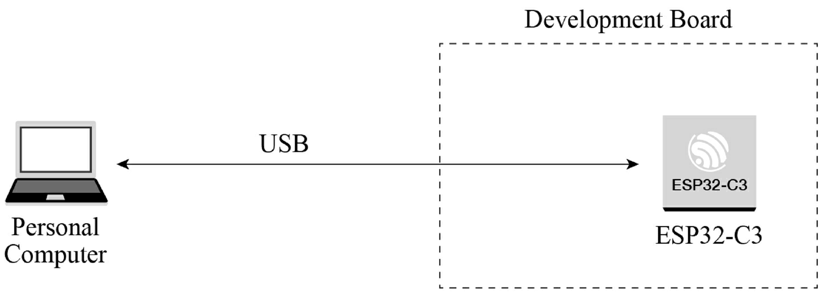
\includegraphics[width=0.65\textwidth]{D5Z/5-16}
    \caption{ESP32-C3 and PC connected through USB Serial/JTAG controller}
\end{figure}

For some ESP32-C3 development boards, a USB-to-UART bridge has been connected to the UART0 interface of the chip. Developers only need to connect the USB interface of the PC to the development board through the bridge, to realise firmware download and log printing, as shown in Figure 5.17.

\begin{figure}[h!]
    \centering
    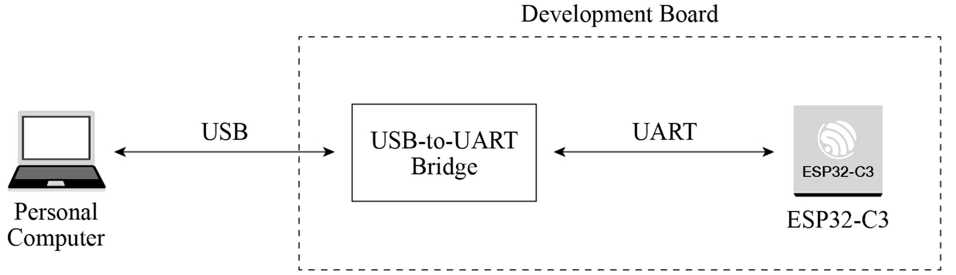
\includegraphics[width=0.65\textwidth]{D5Z/5-17}
    \caption{USB-to-UART bridge connecting ESP32-C3 development board and PC}
\end{figure}

As for a finished board, to save its space and cost, we often use a programmer with USB-to-UART bridge to connect to the UART0 interface on the ESP32-C3 chip, to implement firmware download and log printing. Figure 5.18 shows that a programmer with USB-to-UART bridge is used to connect the development board and the PC.

\begin{figure}[h!]
    \centering
    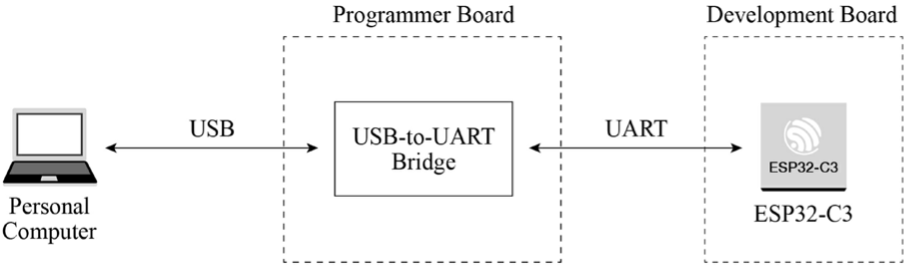
\includegraphics[width=0.65\textwidth]{D5Z/5-18}
    \caption{Programmer with USB-to-UART bridge connecting ESP32-C3 and PC}
\end{figure}

\subsubsection{2. Download firmware.}
The firmware and system parameters of ESP32-C3 are stored in the SPI flash. To flash firmware into the chip, first put the chip in download boot mode. According to Table 5.5, GPIO2 and GPIO8 should be at high level, and GPIO9 should be at low level. Reset the chip to enter download boot mode. Connect ESP32-C3 to the PC using any of the three methods above to start firmware download.

\subsubsection{3. Debug interface.}

There are two ways to debug interface: log printing over serial port and JTAG debugging. 

\begin{term}{Log printing over serial port}
    ESP32-C3 ROM code and IDF SDK output log messages through UART0 by default. Connect ESP32-C3 and the PC with any of the three methods above to enable logging in the PC’s terminal.
\end{term}

\begin{term}{JTAG debugging}
    You can directly use the USB JTAG controller integrated in ESP32-C3 for debugging. To do this, you need to connect the JTAG pins – MTMS/GPIO4, MTDI/GPIO5, MTCK/GPIO6, and MTDO/GPIO7 – to an external JTAG adapter to implement debugging.
\end{term}

\subsection{Guidelines for RF Design}
When designing a smart light product using a module with PCB onboard antenna, pay attention to its placement on the base board to minimize the impact of the board on its antenna performance. The module should be placed as close to the edge of the base board as possible. It’s best to place the PCB antenna area outside the base board and keep its feed point closest to the board.

The antenna feed point of ESP32-C3-WROOM-02 is on the right, while that of ESP32-C3-MINI-1 is on the left. The placement of these two modules is shown in Figure 5.19 and 5.20.

\begin{figure}[h!]
    \centering
    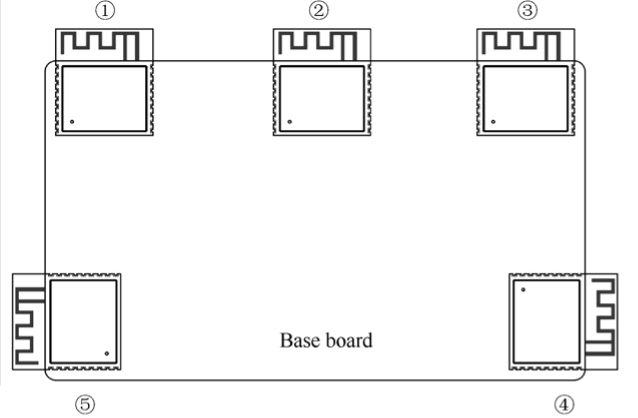
\includegraphics[width=0.6\textwidth]{D5Z/5-19}
    \caption{ESP32-C3 module on base board - antenna feed point on the right}
\end{figure}

\begin{figure}[h!]
    \centering
    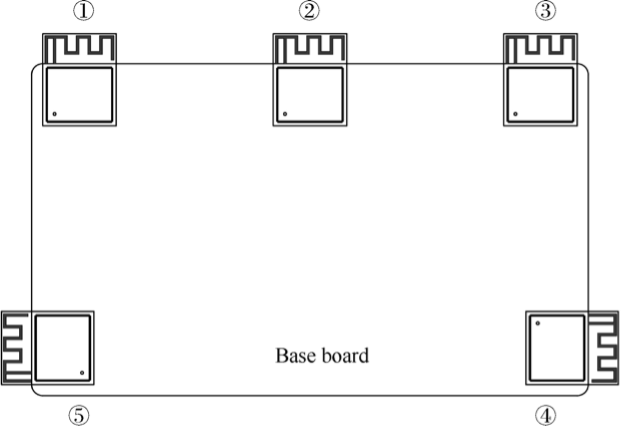
\includegraphics[width=0.6\textwidth]{D5Z/5-20}
    \caption{ESP32-C3 module on base board - antenna feed point on the left}
\end{figure}

\note{For feed points on the right (as in Figure 5.19), position \circled{3} and \circled{4} are preferred. For feed points on the left (as in Figure 5.20), position \circled{1} and \circled{5} are preferred.}

If the positions recommended are unavailable, please make sure that the module is not covered by any metal shell. The PCB antenna area and the area extended by 15 mm should be kept clear, namely no copper traces, wiring, or component placement. The clearance area should be as large as possible, as shown in Figure 5.21. In addition, if there is base board under the antenna area, it is recommended to cut it off to minimize its impact. When designing an end product, pay attention to the impact of enclosure on the antenna.

\begin{figure}[h!]
    \centering
    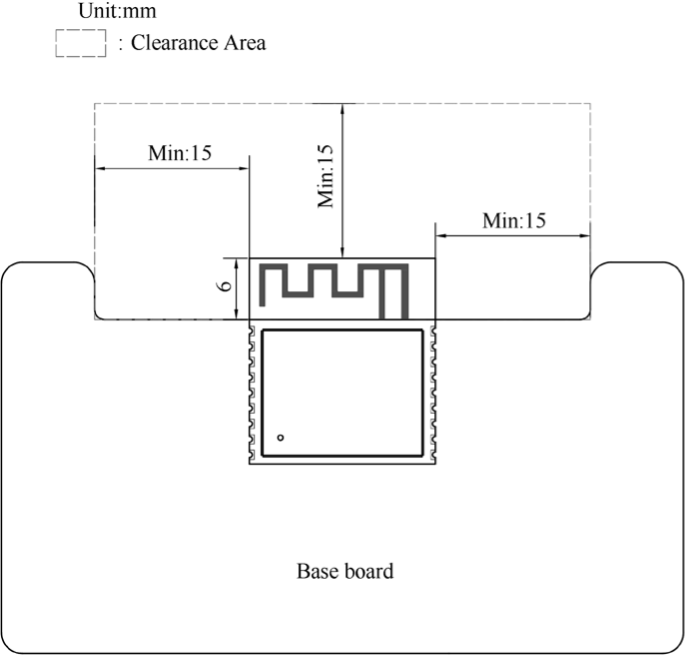
\includegraphics[width=0.5\textwidth]{D5Z/5-21}
    \caption{Clearance area on the base board}
\end{figure}

\subsection{Guidelines for Power Supply Design}
When powering up the ESP32-C3 module through a single pin, the power supply should be of 3.3 V with 500 mA or larger current output. Power ripples can significantly affect the RF TX performance. Generally, the peak value of the ripple should be less than 80 mV when transmitting IEEE 802.11n MCS7 packets, and less than 120 mV when transmitting at 11 Mbit/s.

\section{Summary}
After reading this chapter, you should have acquired knowledge of the following subjects and be able to build your own hardware system for a smart light product:

\begin{itemize}[noitemsep]
    \item Components of a smart light system, implementation of smart light functions, and functional modules of smart LED lights.
    \item Principles and methods of LED dimming and color changing.
    \item Implementing PWM control and wireless communication based on ESP32-C3.
    \item Selecting antenna for wireless communication, and the main parameters and testing methods of Wi-Fi RF performance.
    \item Features of ESP32-C3 and its core circuit design.
    \item Selecting ESP32-C3 module to simplify application design for smart light products.
    \item Guidelines for designing smart light products based on ESP32-C3.
\end{itemize}

\end{document}